% $Id: $
\documentclass[a4paper, 10pt]{article}
% reduced margins
\usepackage{fullpage}
\usepackage[authoryear]{natbib}
% spacing
\usepackage{setspace}
% page headings
\usepackage{fancyhdr}
%\usepackage{lscape}

%\usepackage[nomain,acronym,xindy,toc]{glossaries} % nomain, if you define glossaries in a file, and you use \include{INP-00-glossary}
%\makeglossaries

\usepackage[margin=1.0in]{geometry}
\usepackage{url, subeqn, multirow}
\usepackage{booktabs}
\usepackage{enumerate}

\setlength{\headheight}{15.2pt}
\pagestyle{fancy}
% urls

\usepackage{lscape}
\usepackage{graphicx}
\usepackage{color}
\usepackage{hyperref}
\usepackage{url}
\hypersetup{colorlinks, urlcolor=darkblue}


\usepackage{lscape}
% figs to be 75% of test width
\setkeys{Gin}{width=0.75\textwidth}


%
\renewcommand{\abstractname}{\large SUMMARY}
%
\newcommand{\Keywords}[1]{\begin{center}\par\noindent{{\em KEYWORDS\/}: #1}\end{center}}
%
\makeatletter
\renewcommand{\subsubsection}{\@startsection{subsubsection}{3}{\z@}%
  {-1.25ex\@plus -1ex \@minus -.2ex}%
  {1.5ex \@plus .2ex}%
  {\normalfont\slshape}}
\renewcommand{\subsection}{\@startsection{subsection}{2}{\z@}%
  {-3.25ex\@plus -1ex \@minus -.2ex}%
  {1.5ex \@plus .2ex}%
  {\normalfont\bfseries\slshape}}
\renewcommand{\section}{\@startsection{section}{1}{\z@}%
  {-5.25ex\@plus -1ex \@minus -.2ex}%
  {1.5ex \@plus .2ex}%
  {\normalfont\bfseries}}
\makeatother
%
\renewcommand\thesection{\arabic{section}.}
\renewcommand\thesubsection{\thesection\arabic{subsection}}
\renewcommand\thesubsubsection{\thesubsection\arabic{subsubsection}}
%
\renewcommand{\headrulewidth}{0pt}

\usepackage{listings}

\newenvironment{mylisting}
{\begin{list}{}{\setlength{\leftmargin}{1em}}\item\scriptsize\bfseries}
{\end{list}}

\newenvironment{mytinylisting}
{\begin{list}{}{\setlength{\leftmargin}{1em}}\item\tiny\bfseries}
{\end{list}}

\usepackage{listings}

\definecolor{darkblue}{rgb}{0,0,0.5}
\definecolor{shadecolor}{rgb}{1,1,0.95}
\definecolor{shade}{rgb}{1,1,0.95}


\lstset{ %
language=R,   % the language of the code
basicstyle=\footnotesize, % the size of the fonts that are used for the code
numbers=left,   % where to put the line-numbers
numberstyle=\footnotesize, % the size of the fonts that are used for the line-numbers
stepnumber=1	00,   % the step between two line-numbers. If it's 1, each line 
    % will be numbered
numbersep=5pt,   % how far the line-numbers are from the code
backgroundcolor=\color{shade}, % choose the background color. You must add \usepackage{color}
showspaces=false,  % show spaces adding particular underscores
showstringspaces=false,  % underline spaces within strings
showtabs=false,   % show tabs within strings adding particular underscores
frame=single,   % adds a frame around the code
tabsize=2,   % sets default tabsize to 2 spaces
captionpos=b,   % sets the caption-position to bottom
breaklines=true,  % sets automatic line breaking
breakatwhitespace=false, % sets if automatic breaks should only happen at whitespace
title=\lstname,   % show the filename of files included with \lstinputlisting;
    % also try caption instead of title
escapeinside={\%*}{*)},  % if you want to add a comment within your code
morekeywords={*,...}  % if you want to add more keywords to the set
}

%
\title{Which Came First? The Chicken, The Egg or The Tortilla}
%
\author{Laurence T. Kell\footnote{ICCAT Secretariat, C/Coraz\'{o}n de Mar\'{\i}a, 8. 28002 Madrid, Spain; ~Laurie.Kell@iccat.int; ~Phone: +34 914 165 600 ~Fax: +34 914 152 612.}~,
       Jean-Marc Fromentin\footnote{IFREMER - UMR EME 212, Av. Jean Monnet, 34200 S\`ete, France;~jean.marc.fromentin@ifremer.fr; ~Phone: +33 499 57 32 32 ~Fax: +33 499 57 32 95.}~ and 
       Cody S. Szuwalski\footnote{School of Aquatic and Fishery Science, Box 355020, University of Washington, Seattle, WA, 98195} 
       }
 
%
\date{}
%
\begin{document}


\onehalfspacing
\lhead{\normalsize\textsf{SCRS/2014/025}}
\rhead{}

\maketitle
% gets headers on title page ...
\thispagestyle{fancy}
% ... but not on others
\pagestyle{empty}

%
\begin{abstract}

\textit{
In this paper we look for evidence of a stock recruitment relationships for bluefin, yellowfin and albacore tuna.
Evidence of the existence of a SRR for any of the stock was weak and
the data instead appear to support the argument that recruitment fluctuates around a 
mean level for a period and then a regime shift occurs. This has obvious important implications for 
stock assessment and management advice.}


\end{abstract}

\Keywords{albacore, bluefin, yellowfin, recruitment, spawning stock biomass, stock recruitment relationships, stock assessment,
management, eggs, onions, chickens}

\tableofcontents
\newpage

\section{Introduction}


That there is a stock recuitment relationship (SRR) is a main assumption of many stock assessment models. Management advice 
based on reference points and projection are highly sensitive to the estimated or assumed functional 
form and parameters of the SRR. The SRR is also 
often the only form of density dependence assummed in stock assessment models despite the fact that it can occur in many 
biological processes \cite{lorenzen2002density}
and in different forms; mainly because it is difficult to detect in practice \citep{sinclair_measuring_2002}. 
This is despite the fact that the need for caution in selecting the type of density dependence and specifying its parameters has 
long been recognised in population ecology.

Density dependence is used to stabilise population models has important effects on 
extinction risks \cite{ginzburg1990reconstructibility} and population growth rates \cite{hassell1975density} 
and hence on limit and target reference points If population growth is driven solely by density independent factors 
then a population will shown a random walk and, no matter how severely the vital rates fluctuated around their long term averages, 
the population would eventually increase or decrease without bound \cite{may1986search}.

The information in stock assessment data sets is seldom sufficient to derive the relationship between stock 
and recruitment \cite{lee2012steepness}. It has also been known for nearly a century 
\citep{hjort_fluctuations_1926} that fish stocks can fluctuate extensively over a large range  of spatial and temporal 
scales independent of human exploitation. \cite{gilbert_towards_1997} argued that recruitment may shift between 
regimes independently of stock biomass and that spawning stock biomass (SSB) is a function of recruiment. 
Periods of high or low recruitment generate periods of high or low stock biomass respecitively as fish mature. 

What came first? the need of stock assessment working groups for a stock and recruitment relationships to make 
the tortilla, (i.e. fitting  statistcally integrated models, deriving reference points and making stock projections) or 
evidence that stock biomass drives recruitment. 

Determing the relationship between stock and recruitment is complicated by the fact that values of stock and recruitment 
used in most analyses are based on stock assessment data sets where SSB is used as a 
proxy for spawning  potential (SRP). SSB assumes that fecundity is proportional to mass-at-age irrespective of the demographic 
composition of adults and that processes such as maturity are simple functions of age. However, changes in growth and egg 
production (EP) are well documented and may impact on productivity and hence reference points and management advice 
(see Kell at al. submitted). Recruitment is not measured but estimated along with mortality (Z) which may
involve fixing natural mortality (M), since M is a difficult parameter to actually estimate \cite{lee2012steepness}.
However if M varies with time (e.g. due to the environment or density dependence) then the estimated stock
recruitment relationship assuming M is time invariant will be biased. For example \cite{nash2009stock} estimated a Ricker SRR 
for North Sea herring, which disappeared when natural mortality was allowed to vary over time (Kell et al. submitted).

\section{Material and Methods}

We explore non-parameteric stock recruitment relationship, auto-correlation in recruitment,
cross correlations between recruiment and SSB and regime shifts for stock and recruit time series
obtained from age based ICCAT stock assessments

\subsection{Data}

Time series of SSB and recruitment were obtained from the most recent ICCAT stock assessments for North Atlantic albacore (ref), 
the Eastern and Western Altantic bluefin tuna stocks (ref) and yellowfin tuna (ref). The albacore assessment was conducted using
Multifan-CL \cite{fournier_multifan-cl} with no constraint on the SRR parameters. For the other stocks
the assessment was based on virtual population analysis (VPA) again with no constraint on the SRR. In the case of Western Altantic bluefin
two catch time series were considered, i.e. the reported catches and an inflated catch series which allowed for the misreporting 
of catch levels.

\subsection{Methods}


\subsubsection{Stock Recruitment Relationships}

The Beverton and Holt SRR \citep{beverton_dynamics_1993} is derived from a simple density dependent mortality model
where it is assumed that mortality of pre recruits is proportional to their density and the number of recruits 
increases towards an asymptotic level ($R_{max}$) as egg production increases. 

The Ricker SRR assumes that density dependent mortality is proportional to the initial number of eggs or larvae. 
This may be appropriate when a prey species is temporarily massed in 
unusual numbers and the number of prey eaten depends on the abundance of predators, 
but not on the abundance of prey. Hence such situations cannot last long, and the predators cannot make the prey in question their principal
yearly food, \cite{ricker1987computation}. Alternative mechanisms 
include cannibalism, habitat limitations, and aggregation 
\citep{rose2001compensatory,brooks2007generalized,powers2004recruitment}. 

The majority of fisheries stock assessment modelling is parametric. However when modelling 
the relationship between stock and recruitment models may not adequately explain the data or the data may not
informative enough to estimate the parameters \cite{hillary2012multi}. Therefore we fitted a LOESS smoother 
\citep{cleveland1992local} to allow the relationship between stock and recruitment to be explored without specifying 
in advance the assumed process (i.e. compensation, over compensation or depensation) as required when fitting one of 
the standard functional forms. We then look for patterns in the residuals that may indicate that other processes
influence recruitment.

\subsubsection{Cross correlations}

In order to evaluate whether there is a monotonic relationship between recruitment and SRP (see Szuwalski et al, submitted) 
cross correlations were calculated based on Spearman's correlation \citep{spearman1904general}. If there is compensation
(for example recruitment follows a Beverton and Holt stock recruitment relationship) then there will be a significant 
correlation equal to the age at recruitment. \\
\textbf{[\textit{The significance levels in the plots are probably wrong due to auto-correlation in the time series.
2 options either to i) remove the CI or ii) calculate new corrected ones based on \cite{pyper1998comparison}}]}

However if stock biomass is driven by recruitment as a result of fluctuations in the 
environment \citep{gilbert_towards_1997} then there will be negative lags at corresponding to the mature ages. 
Only if SSB has a larger and significant influence on recruitment than recruitment does on SSB 
then is the existence of a S-R is supported (Szuwalski et al, submitted). 

\subsubsection{Regime Shifts}

Evidence for regime shifts are explored using a a sequential t-test algorithm 
(STARS; \cite{rodionov2004sequential}) as modified by Szuwalski et al., (submitted)


\section{Results}

Time series of recruitment and SSB are shown in \textbf{Figure} \ref{rec} and \ref{ssb}. Recruitment is then plotted against SSB along with 
a non-parameteric LOWESS fit in \textbf{Figure} \ref{sr}. The residuals to the fits are shown in \textbf{Figure} \ref{rsd}.
Results for Eastern Atlantic bluefin series based on the inflated catch are in red.

Auto correlation in the recruitment time series are evaluated by plotting correlogrammes in \textbf{Figure} \ref{acf} for recruitment
and for recruitment residuals from the non-parameteric fits in \textbf{Figure} \ref{acf2}; non-randomess can be investigated
by comparing correlations by lag with the upper and lower bounds at the 5\% significance level. 

To check the assumption that there is monotonic relationships between recruitment and SSB (e.g. a Beverton and Holt stock recruitment relationship 
without over compensation) the cross Spearman correlations are plotted in \textbf{Figure} \ref{ccf}; again non-randomess can be investigated
by comparison with the 5\% significance levels. For yellowfin the righhand limb of the Ricker curve was due to the early points in the
time series, these were removed prior to calculating the cross correlations.

Sequential t tests for regime shifts \cite{rodionov2004sequential} in recruitment are shown in \textbf{Figure} \ref{stars} and 
for recruit residuals from the non-parameteric fits in \textbf{Figure} \ref{stars2} and in  \textbf{Figure} \ref{stars3} for SSB.

\begin{description}
 \item[The Relationships between Recruitment and Stock] is explored in \textbf{Figure} \ref{sr}.
 A Ricker stock recruitment relationship is suggested for yellowfin, however the points on the righthand 
 limb of the Ricker curve all come from the early period of the time series and could also be
 explained by a regime shift. For albacore a Beverton and Holt or Ricker for albacore could
 be fitted to the data. For the bluefin time series the picture is less clear. For 
 the eastern stock low recruitments are seen with higher levels of SSB, which could be consistent with
 over compensation. For the western stock, recruitment declined year-on-year from the start of 
 the time series until stablising in recent years to a low level about which recruitment has fluctuated.
 
 \item[Residual patterns]  in \textbf{Figure} \ref{rsd} shows a systematic pattern, in that recruitment
 in the early years was lower than predicted. There is no systematic pattern in the albacore residuals.
 For eastern bluefin recent recruitment is lower than the predicted values, this is a result of the under reporting
 of catches on the VPA estimates. For Western bluefin in the mid period, when recruitment was declining year-on-year the 
 residuals are all positive.  
 \textbf{Figures} \ref{sr} and \ref{rsd} indicate problems with all the fits apart from albacore. 
 
 \item[Autocorrelation] plots in \textbf{Figure} \ref{acf} show significance autocorrelation for all time series other
 than albacore. In the albacore assessment recruitment deviates were estimated as a random walk and so autocorrelation was
 removed from the residuals. 
 The residuals from the non-parameteric fits show less autocorrlation  (\textbf{figure} \ref{acf2}) since
 the smoother has removed some of the trends since recruitment and SSB are correlated as
 seen by the cross correlations.
 
 \item[Cross correlation] plots (\textbf{figure} \ref{ccf}) do not support recruiment being
 driven by SSB, since there a a lag of 1 for recruitment (i.e. at age 1) with SSB is no more important than other lags. 
 For Eastern Atlantic bluefin
 the cross correlations are negative with lags less than 1 being the most significant. If there was overcompensation
 then there should be a significant negative correlation with a lag of 1. The cross correlations therefore do not support
 the existence of a stock-recruitment relationship. 
 Teleosts generally produce a large number of eggs with only a small number survive to recruitment. 
 This has nothing to do with fishing since the stock recruitment relationship only considers the pre-exploitation stage and fishing 
 reduces the spawning stock not recruitment. Therefore positive lags are not affected by fishing. However, negative lags
 are as the numbers surviving to maturity are determined by mortality levels.
 
 \item[Regime shifts] are explored in \textbf{Figures} \ref{stars} and  \ref{stars2} overlay the regime shifts on the recruitment and recruit residual time 
 series. If it is believed that there is no stcok recruiment relationship then in all stocks there are regime shifts (i.e.
 in both the mean and variance) in recruitment about every 10 years.
 The regime shifts in SSB for Western Atlantic bluefin and yellowfin coincide with those in recruitment. However, the regime shifts
 in Eastern bluefin and albacore show large variatons which do not obviuously coincide with those in recruitment.
\end{description}

\section[Discussion]{Discussion}

The results show that evidence supporting the existence of a SRR for any of the stock is weak and
instead appear to support the argument of \cite{gilbert_towards_1997} that recruitment fluctuates around a 
mean level for a period and then a regime shift occurs. This has obvious important implications for 
stock assessment and management advice provided by ICCAT and other Regional Fisheries Management
Organisations (RFMOs).

\begin{description}

\item[Quantification of uncertainty in stock assessments]

The SCRS provides advice on management measures within the Kobe framework, which includes integrating
various scenarios based on key uncertainties e.g. about recruitment processes and SRR assumptions. 

For the Western bluefin stock there two scenarios are considered when providing advice, i.e.
either a Beverton and Holt or segmented regression SRR. Both assume that dynamics are stationary i.e. 
that the dynamics are ``either or`` and the main issue is to identify which are the true dynamics rather 
than that there may have been a change in the dynamics. However, recent work now suggests that there 
has been a regime shift \cite{fromentin2013oceanographic}.

For the Eastern bluefin stock two scenarios were considered for historic catch levels (i.e. reported and inflated)
and three for future recruitment levels (i.e. low, medium or high re-sampled from different periods of the historic 
series). From the VPA estimates of SSB and recruits 
it could be argued that the SRR is of a Ricker functional form and that the stock is has always been on the right-hand
limb of the Ricker curve. 
However it is hard to find a biological explanation to support this argument especially as there appeared to be no
relationship between SSB and recruitment. The analysis would suggest instead that there has been
a series of regime shifts. 

In the case of the Eastern and Western stocks the complex evolution of the bluefin fisheries and the use of
VPA to estimate recruitment and SSB from reported catches means that it is difficult to
understand the actual processes.

For yellowfin and albacore no stock recruitment hypotheses were considered when developing scenarios. Albacore
was assessed using Multifan-CL \cite{fournier_multifan-cl} and there was no significant relationship between SSB and
recruitment. The yellowfin assessment was conducted using VPA, which does not involve a stock recruitment relationship
and the projection to provide advice on catch quotas assumed constant recruitment, i.e. that there was no SRR.

Advice for the case study stock is based assuming stationarity.
However, the evidence of regime shifts in the data means that it is important to provide advice on 
that takes into account changes in recruitment dynamics and the consequences of a transition from 
current recruitment levels to higher or lower levels rather than to determine the 'corrrect' recruitment 
model or to combine several models when providing advice. 


\item[Characterisation of quality of the fisheries data and biological information]

This simple study showed that there is considerable uncertainty about the knowledge of
key biological processes and that current advice is unlikely to be robust to that uncertainty.
Especially since recruitment processes are assumed to be stationary and estimates of
SSB assume time invariant growth and fecundity.

\item[Limit Reference Points, Harvest Control Rules,  and Management Strategy Evaluations]

Reference points should be evaluated as part of a feedback HCR using MSE where Operating Models (OMs)
are conditioned on hyotheses about the stock recruitment dynamics. This will allow robust HCR and
reference points to be developed

\item[Incorporation of Ecosystem, Climate, and Habitat (ECH) information into stock assessments]

The ability of management strategies to achieve management goals are impacted by environmental variation, \cite{punt2013fisheries}
in a review found that most studies showed that 
modifying management strategies to include environmental factors does not improve the ability to achieve management goals
much, if at all, and only if the manner in which these factors drive the system is well known. They concluded that until the skill of 
stock projection models improves, it seems more appropriate to consider the implications of plausible broad forecasts related to how
biological parameters may change in the future as a way to assess the robustness of management strategies, rather than attempting
specific predictions.

\end{description}

\section{Conclusions}

Most stock assessment models implicitly assume some types of density dependence. For example surplus production (either 
explicitly in a biomass dynamic model \cite{pella_generalized_1969} or implicitly when performing an age based projection with 
a SRR or constant recruitment) means that there is an equilibrium population abundance, K or $B_0$, which if the
population falls below K the population growth rate (r) will on average be greater than 1 and in the abscence of fishing the 
population will increase. Alternatively if the population grows above K r will fall below 1 and the population will decline. 

However if the population is subject to "systemic" pressure \cite{Shaffer1981} such as a regime shift then assuming density-dependent 
regulation may cause an underestimation of the risk of decline or result in forgone yield. The population may be subject to
trends due to a change in survival rates or fecundities in which case it may not be appropriate to use density dependence 
models such as Ricker, Beverton-Holt, logistic, etc.  

\cite{overland2010climate} pointed out that ecosystem variability can involve a variety of climate to
ecosystem transfer functions. These can be expected to convert red noise of the physical system to redder
(lower frequency) noise of the biological response, but can also convert climatic red noise to more abrupt and
discontinuous biological shifts, transient climatic disturbance to prolonged ecosystem recovery, and perhaps
transient disturbance to sustained ecosystem regimes. All of these ecosystem response characteristics are likely
to be active for at least some locations and time periods, leading to a mix of slow fluctuations, prolonged trends,
and step-like changes in ecosystems and fish populations in response to climate change. Which provide
challenges for management advice.

A solution is to use Management Strategy Evaluation (MSE) to develop management strategies that are robust to
uncertainty about the recruitment and stock dynamics dynamics. 
This requires the development of Operating Models (OMs) to simulate the main uncertainties about system dynamics and 
to test the performance  of alternative management strategies. MSE involves a number of steps \cite{punt_developing_2007} i.e.

\begin{itemize}
 \item identification of management objectives and mapping these to performance measures in order to quantify how well they have been achieved.
 \item selection of hypotheses about system dynamics.
 \item conditioning of OMs on data and knowledge and possible rejecting and weighting the different hypotheses.
 \item identifying candidate management strategies and coding these up as MPs %(i.e.the combination of pre-defined data, together with an algorithm to which such data are input to set control measures).
 \item projecting the OMs forward using the MPs as feedback control procedures; and
 \item agreeing the MPs that best meet  management objectives.
\end{itemize}

The performance of management strategies and hence the eventual selection of the strategy to be implementation depends upon the hypotheses
included in the OM. The choice of scenarios for use in provision of management advice is therefore critical. In the case studies the 
scenarios are not consistent across stocks.
In some cases the scenarios were selected from assessment runs which had been initially been conducted as
sensitivity tests to evaluate the relative importance of model assumptions. 

Scenarios should include ones for which it is important that management advice is robust to. For example the occurrence 
of regime shifts. Therefore management strategies evaluated should include ones which can 
respond to regime shifts, i.e. allow for non-stationarity. This will allow the robustness of current advice to be evaluated
and alternative strategies to be developed.

Fisheries independent time series of  recruitment and spawning stock biomass will of extreme importance in better understanding
the relationship between recruitment and spawning reproductive potential.


\newpage
\bibliography{refs.bib} 
\bibliographystyle{abbrvnat} 

\newpage\clearpage\section{Figures} 

\begin{figure}[!ht]\begin{center} 
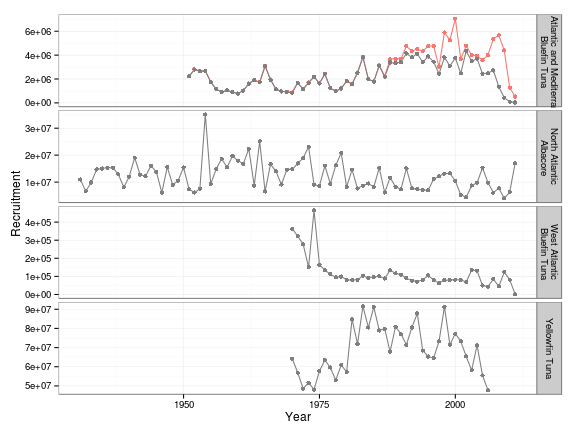
\includegraphics{figs/sr-rec.png}
\end{center}
\caption{\bf{Time series of recruitment; the red lines repesent the Eastern Atlantic bluefin series based on the inflated catch.}}
\label{rec}\end{figure} 

\begin{figure}[!ht]\begin{center} 
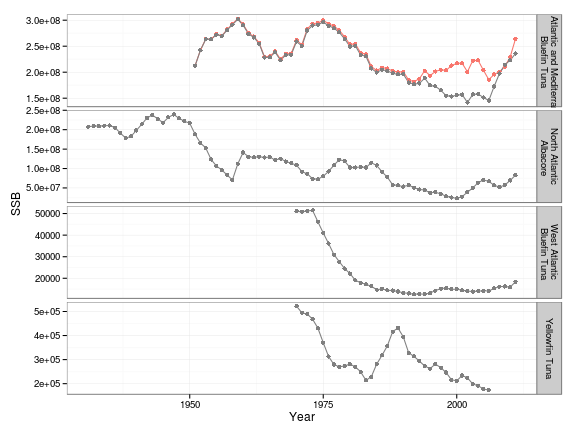
\includegraphics{figs/sr-ssb.png}
\end{center}
\caption{\bf{Time series of Spawning Stock Biomass}}
\label{ssb}\end{figure} 

\begin{figure}[!ht]\begin{center} 
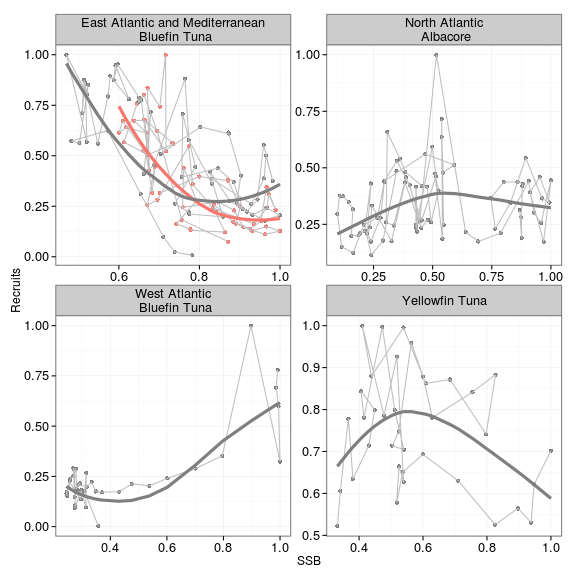
\includegraphics{figs/sr-np-sr.png}
\end{center}
\caption{\bf{Plots of Recruitment against Spawning Stock Biomass, with non-parameteric fits using a LOWESS smoother.}}
\label{sr}\end{figure} 

\begin{figure}[!ht]\begin{center} 
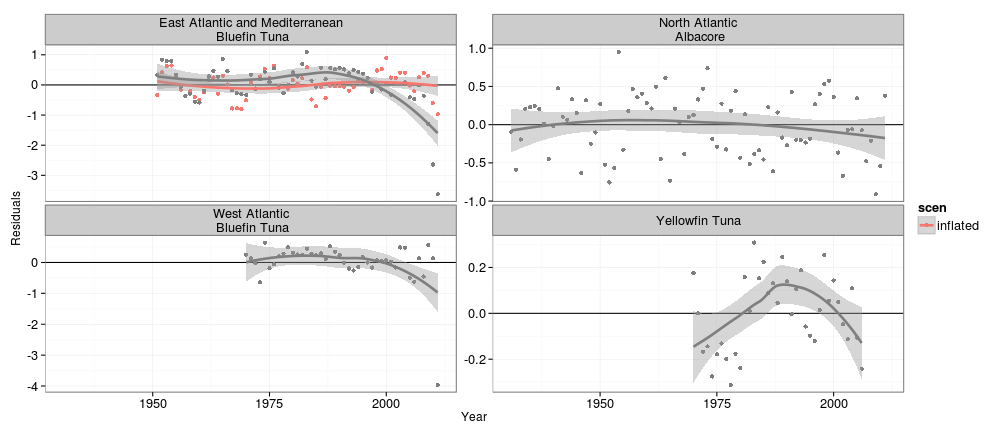
\includegraphics{figs/sr-np-rsd.png}
\end{center}
\caption{\bf{Plots of residuals from non-parameteric fits to Recruitment as a function of Spawning Stock Biomass.}}
\label{rsd}\end{figure} 

\begin{figure}[!ht]\begin{center} 
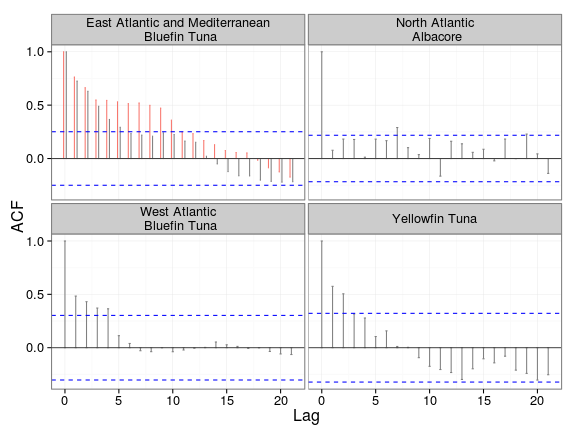
\includegraphics{figs/sr-acf-rec.png}
\end{center}
\caption{\bf{Plots of recruitment auto correlation, horizontal lines are the 5\% CIs}}
\label{acf}\end{figure} 

\begin{figure}[!ht]\begin{center} 
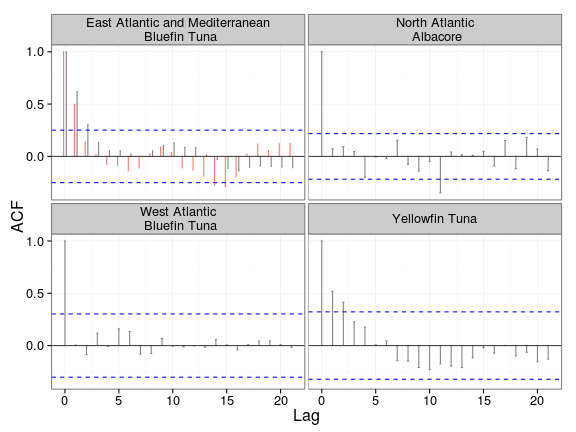
\includegraphics{figs/sr-acf-rsd.png}
\end{center}
\caption{\bf{Plots of recruitment residuals auto correlation, horizontal lines are the 5\% CIs}}
\label{acf2}\end{figure} 

\begin{figure}[!ht]\begin{center} 
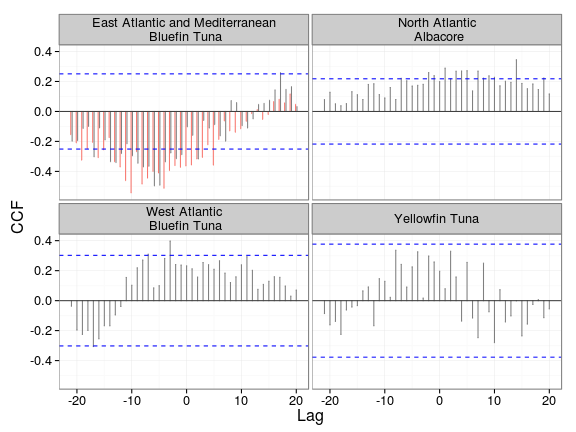
\includegraphics{figs/sr-cc-sr2.png}
\end{center}
\caption{\bf{Plots of cross correlation between recruitment and SRP, horizontal lines are the 5\% CIs}}
\label{ccf}\end{figure} 

\begin{figure}[!ht]\begin{center} 
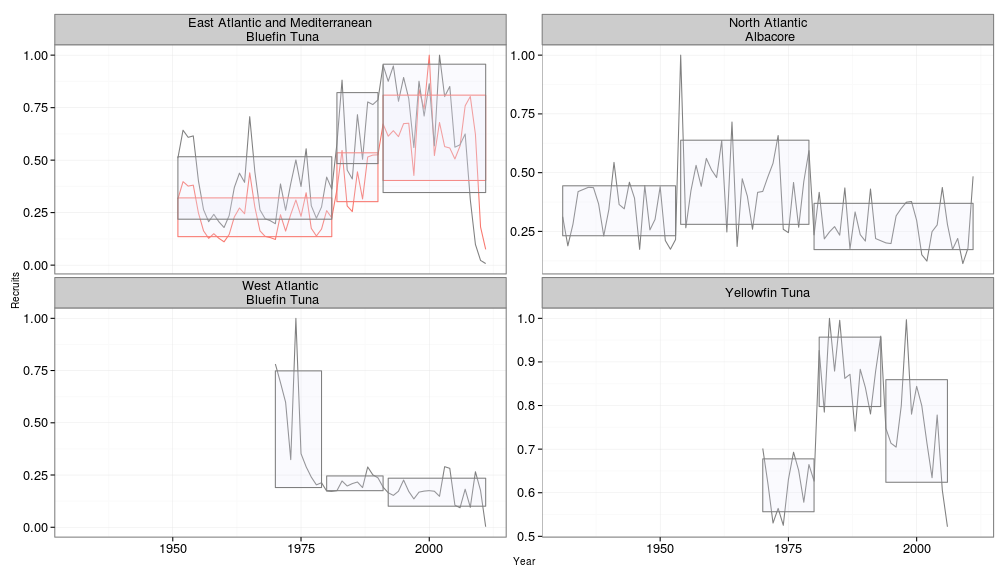
\includegraphics{figs/sr-stars-rec2.png}
\end{center}
\caption{\bf{Recruitment by year Sequential t test for regime shifts (Rodionov, 2004) in recruitment}}
\label{stars}\end{figure} 

\begin{figure}[!ht]\begin{center} 
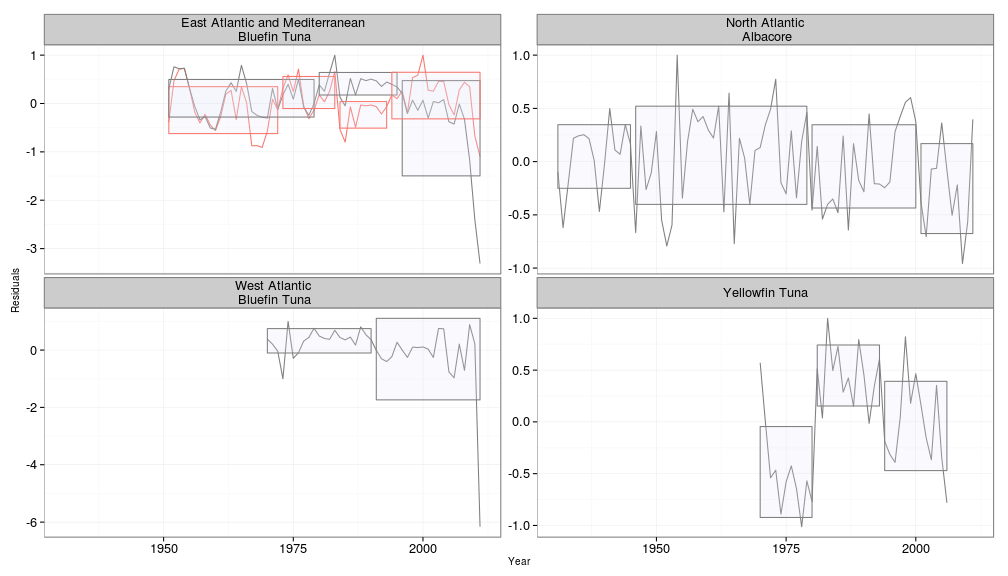
\includegraphics{figs/sr-stars-rsdl2.png}
\end{center}
\caption{\bf{Recruitment by year Sequential t test for regime shifts (Rodionov, 2004) in recruitment residuals}}
\label{stars2}\end{figure} 

\begin{figure}[!ht]\begin{center} 
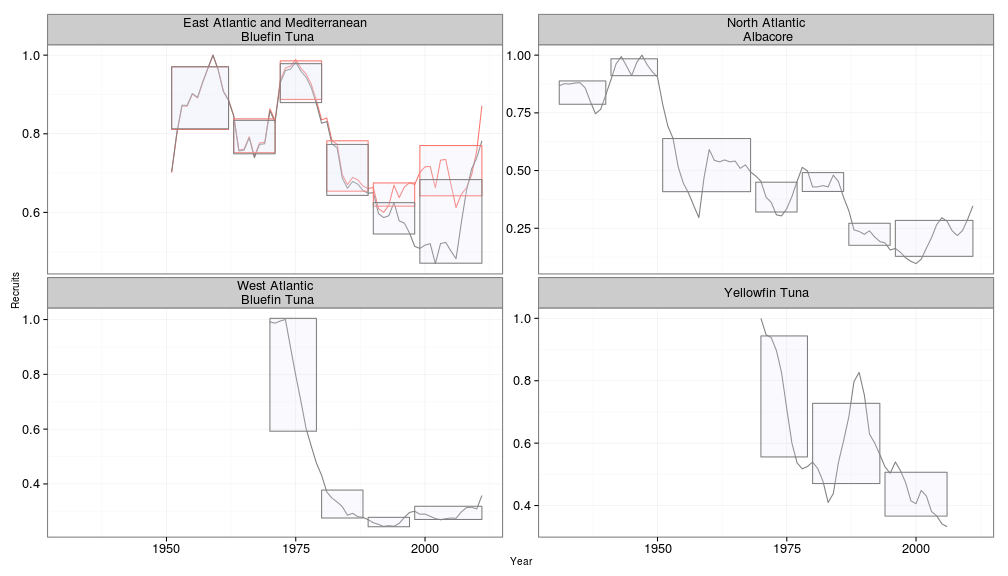
\includegraphics{figs/sr-stars-ssb2.png}
\end{center}
\caption{\bf{Recruitment by year Sequential t test for regime shifts (Rodionov, 2004) in SSB}}
\label{stars3}\end{figure} 


\end{document}

\newpage\clearpage\section{Appendices}
\newpage\clearpage\subsection{\textbf{Appendix 1:} }

\newpage\clearpage\section{Equations}

\begin{table}
\caption{Equations}
\label{tab:datasumm}
\begin{tabular}{lp{10cm}}
\toprule
\toprule

\textbf{Population dynamics} &
 \begin{equation} N_{a+1, y+1} = N_{a,y} e^{-Z_{a,y}} \end{equation} \\
%
 &
 \begin{equation} N_{p,y} = N_{p-1, y-1} e^{-Z_{p-1, y-1}} + N_{p,y} e ^{-Z_{p, y-1}} \end{equation} \\
%
 &  \begin{equation} N_{r,y} = f(B_{y-r}) \end{equation} \\
\midrule

% Mortality rates
\textbf{Mortality rates} & \begin{equation} Z_{a,y} = F_{a,y} + D_{a,y} + M_{a,y} \end{equation} \\
%
 & \begin{subequations} 
\begin{equation} F_{a,y} = \sum_{i=1}^f P_{i,a,y} S_{i,a,y} E_{i,y} \end{equation}
\begin{equation} D_{a,y} = \sum_{i=1}^f \left(1- P_{i,a,y}\right) S_{i,a,y} E_{i,y} \end{equation}
\end{subequations}\\
\midrule

% Catch equation
\textbf{Catch equation} & \begin{equation} C_{f,a,y} = N_{a,y} \frac{F_{f,a,y}}{Z_{f,a,y}} \left(1 - e^{-Z_{a,y}} \right) \end{equation} \\
\midrule

%
\multicolumn{2}{l}{\textbf{Stock recruitment relationships}} \\
\addlinespace
% BH
Beverton \& Holt & \begin{equation} N_{r,y} = \frac{B_{y-r}}{\alpha B_{y-r} + \beta} \end{equation} \\
% BB
\bottomrule

\multicolumn{2}{l}{\textbf{Growth and maturity}} \\
% BH
von Bertalanffy & \begin{equation} N_{r,y} = \frac{B_{y-r}}{\alpha B_{y-r} + \beta} \end{equation} \\
\bottomrule
\end{tabular}
\end{table}

\end{document}


\begin{description}

\item[Quantification of uncertainty in stock assessments]

The Commission expects risk-based advice on management measures as prescribed in the Kobe II 
Strategy Matrix and as embedded in its Decision Framework (Rec. 11-13). An important aspect of providing such scientific 
advice is adequate quantification of uncertainty in stock condition and future prospects under future management option 
scenarios. With the advent of more commonly applied, highly parameterized stock assessment models, the computational 
investment in quantifying uncertainty in stock status and future prospects is quite heavy. This is also the experience 
at other tRFMOs and a number of approximations for quantifying both process and observational uncertainty are being 
applied to develop risk-based management advice. 
\begin{itemize}
 \item Efficient and unbiased approximations of uncertainty in advice 
 \item Graphical presentation of the approximations of uncertainty
\end{itemize}


\item[Characterization of quality of the fisheries data and biological information]

Basis of the Agenda Item. [Res 13-15] Resolution by ICCAT to Complete the Standardization of the Presentation of 
Scientific Information in the SCRS Annual Report: Recalling the recommendation of the Kobe II Workshop of Experts 
to Share Best Practices on the Provision of Scientific Advice that the Executive Summaries of scientific reports 
should be standardized to the extent possible; recalling that the Kobe III Workshop of Experts on Science recognized 
that substantial uncertainties still remain in the assessments and recommended that the Scientific Committees and 
Bodies of the t-RFMOs develop research activities to better quantify the whole uncertainty and understand how 
uncertainty is reflected in the risk assessment inherent in the Kobe II Strategy Matrix;  considering  the utility 
of distinguishing, where possible, between the inherent variability in natural system (i.e. life history parameters) 
which is unavoidable, and the uncertainty related to the quality of the state of knowledge of the system and of the 
fishery data, which could potentially be reduced through improvements to the available data and/or the models applied;
further noting that the SCRS, as part of its 2015-2020 Strategic Plan for Science, will develop specific formats to 
provide scientific advice in line with the needs of the Commission. 


\begin{itemize}
 \item Providing clear, transparent, and standardized procedures to produce qualitative scores on input data and assumptions
\end{itemize}

\item[Reconcile the results when dealing with Multiple Modeling Methods]

There is a trend in recent assessments conducted by the SCRS to use multiple
modelling methods to estimate the status of the stock relative to ICCAT conservation benchmarks. While WGSAM agrees the use 
of multiple approaches is a good practice, situations have arisen where the different methods give results that are not 
consistent yet equally plausible (see, for example, ICES 2007).

\begin{itemize}
 \item Model ensemble approaches to stock assessments
 \item Combining and articulating results from multiple models
 \item Appropriate weighting of results across different models and modeling platforms
\end{itemize}


\item[Limit Reference Points, Harvest Control Rules,  and Management Strategy Evaluations]

The evaluation of Limit Reference Points (LRP) and Harvest Control Rules (HCR) through 
the use of Management Strategy Evaluation (MSE) is increasingly being recognized by global tuna RFMOs as an 
effective means to advance their fishery management process. The 2013 assessments of albacore and swordfish
were used as examples of how an MSE process could possibly be formally included in the management of those stocks.
The WGSAM plans to continue this effort by (1) continuing to refine the methods within the MSE process, (2) 
introduce MSE more assessments when and where appropriate, and (3) foster lines of communication that keep 
managers informed of their benefits and weaknesses. Regarding dialog and communication, ICCAT has recently 
adopted the [Rec. 13-18] Recommendation by ICCAT for Enhancing the Dialogue Between Fisheries Scientists and 
Managers that aims to enhance communication and foster mutual understanding between fisheries managers and 
scientists in order to facilitate more streamlined, science-based decision-making. As well, the Recommendation
outlines specific tasks to be achieved during the first meeting of the Standing Working Group for Enhancing 
the Dialogue Between Fisheríes Scientists and Managers (SWGSM) in 2014.


\begin{itemize}
 \item Comparison of MSE approaches within stock assessments
 \item MSEs that demonstrate the efficacy of the ICCAT harvest Control Rule
 \item Recommendations on the continued use of MSE and stock that could likely benefit from their use
 \item Implementation of the Precautionary Approach in the ICCAT arena through reference points, harvest controlrules, and other elements of harvest strategies
 \item Biological factors to be considered in defining Harvest Control Rules
 \item Sources of variability and uncertainties
\end{itemize}


\item[Incorporation of Ecosystem, Climate, and Habitat (ECH) information into stock assessments]

The manner in which ECH considerations can be included into the fishery management 
decision making process is very broad and varied.  At one end of the spectrum are purely qualitative approaches
with the simple acknowledgement of these processes exist and modulate fish population dynamics.  At the other 
end of the spectrum are formal quantitative approaches.  Quantitative approaches generally seek to use ECH 
either to directly adjust selected model parameter values or as index data intended to indirectly guide the 
direction of several estimated parameters or an overall trend in the simulated population.   Neither qualitative
nor quantitative methods should be viewed as superior to the other as the suitability of each is situation specific.


\begin{itemize}
 \item Qualitative methods of enhancing stock assessments and/or management advice through the use of ECH considerations
 \item Quantitative methods of enhancing stock assessment and reducing uncertainty
 \item Communication of the effects of ECH on fish population dynamics to managers
\end{itemize}

\end{description}


A stationary time series should have no significant autocorrelations after the first few lags (e.g. 1 or 2), 
while in contrast a non stationary time series will have significant autocorrelations over a range of lags. 
A visual test for stationarity is therefore to plot the correlogram (plots of the autocorrelation against lag). 
A formal test for stationarity whether the data sets are sufficiently informative to be sure whether they are 
stationary or not is the Kwiatkowski Phillips Schmidt Shin (KPSS,\cite{kwiatkowski_testing_1992}). 


Good goal, my friend, this is simple and right to the point!!
I think it is largely sufficient for a SCRS paper and there is a good  
basis for a per review one...

Regarding the methods, I have one main THOUGHT: When you looked at the  
cross-correlations, I don't think you can rely on the CI given by the  
R function, because this function probably assumes that the  
observation of each series are independent, ie without any  
autocorrelation, which is known to strongly bias the ddl... One way to  
go this common problem is to recalculate the real ddl through some  
correction (I used this proposed by Pyper & Peterman in CJFAS in 1998)  
or more simply to remove these CI and just look at the sign and  
amplitude of the cross-correlations.

I was also thinking about comparig the dates of the regime shifts  
detected in the Rec and SSB time series. In theory, that coud be  
another way to distinguish between the egg and the chicken, but as  
most of the series come from VPA, we are fucked... too bad...

About the text, I few things:
The last two lines of the intro are a bit bizarre (remove or rephrase,no?)

You include auto-correlation function under the hat of stationarity. I  
see the point, but the research of regime shift is more directly a  
detection of non stationarity (order 1) than autocorrelation profiles,  
don't you think? Actually, I won't mention stationarity in hte  
Methofs, but only in results and discussion as a general outcome of  
the analyses.

Finally, there is one thing THAT YOU CANNOT CHANGE: THe title!!! it is  
just PERFECT!! The Monthy Python would have found a better one!!!!

BY the way, you don't have to put me in to co-authors, I did  
nothing... but will be happy to contribute to the extension of such  
work!

Cheers,
JM



  